\documentclass{article}

\usepackage{graphicx}
\usepackage{epsfig}
\usepackage{float}
\usepackage{booktabs}

\title{Evoker: a genotype visualization tool}
\author{Jeffrey Barrett (\texttt{barrett@sanger.ac.uk})\\
James Morris (\texttt{jm20@sanger.ac.uk})}
\date{\today}

\begin{document}

\maketitle

\section{Introduction}

Evoker is a tool designed for visualizing genotype cluster plots as part of quality control procedures for genome-wide association studies. It provides a solution to the computational and storage problems related to being able to work with the huge volumes of data generated by such projects.

\section{Getting started with Evoker}

Using Evoker requires two important parts: the data, formatted and named in a specific way, can be stored either locally or on a remote server to which you have SSH access and the main Evoker program, which is run locally on your PC and is used for displaying cluster plots and assigning them a Pass/Fail verdict. You will need Java 5.0 (also known as version 1.5) or newer on your local machine to run Evoker. There are three platform specific Evoker installation bundles for Mac, Windows and Linux and an additional package which combines all three. All the different packages contain the same perl scripts and example files but simply differ in the type of file used to start the Evoker program. The Mac bundle contains an application called Evoker, the Windows bundle contains the executable file \texttt{Evoker.exe} and the Linux bundle contains a jar file called \texttt{Evoker.jar}. On all platforms to start Evoker simply requires double clicking on the relevant Evoker icon, in the case of Mac and Windows launching Evoker in this way starts the program with additional memory enabling the loading of larger studies. Launching Evoker by double clicking the \texttt{Evoker.jar} file starts the program with the default amount of memory which may be insufficient for larger data sets. If double clicking the Evoker icon does not work or extra memory is required then Evoker can be launched from the command line by issuing the following command:
\begin{verbatim}
java -jar Evoker.jar -Xmx 1024m 
\end{verbatim}
This will launch Evoker with up to 1Gb of memory available, to increase this amount further simply change the value passed to the \texttt{-Xmx} argument, this approach also works on Mac and Windows using the \texttt{Evoker.jar} file.

\subsection{File formats and conventions}

Evoker can work with files formatted in two different ways, either using a default file format based around the binary style files of the widely-used \texttt{PLINK} program or an Oxford file format that is based on the files used in the \texttt{WTCCC2} project. 

In both cases the data for your project (whether stored locally or remotely) should all be kept in a single directory to which you have read and write access. Because Evoker understands how to load and parse your data based on which files are in this directory you should not have any other files inside that directory. The files in this directory are organised by `collection' (a group of samples) and `chromosome' (a group of SNPs).

The collection groupings can be any subset of your data which you wish to plot separately, such as case and control samples, or samples genotyped in different laboratories. Furthermore, `chromosomes' can really be any grouping of SNPs, as this designation is used mostly for bookkeeping by the program. Indeed, you could organise your data with only a single `genome' chromosome, requiring only one set of files per collection, but this will result in a performance loss when using Evoker.

% intensity format table
\begin{table}
  \begin{center}
    \caption[Intensity file formats]{Intensity file formats}
    \vspace{0.2cm}
    \label{FileFormats}
    \begin{tabular}[p]{ l l l}
     \toprule[1.5pt]
      Data format & Input file & int2bnt.pl command line argument \\
      \midrule
		Default format & input intensity file & \texttt{int2bnt.pl}\\
		Illuminus & input intensity file & \texttt{int2bnt.pl --filetype illuminus}\\
		Chiamo (v0.1 and v0.2) & input intensity file & \texttt{int2bnt.pl --filetype chiamo}\\
		BeagleCall & allele signals file (.signals) & \texttt{int2bnt.pl --filetype beagle}\\
		Birdsuite & allele\_summary file & \texttt{int2bnt.pl --filetype affy}\\
      \addlinespace      
      \bottomrule[0.5pt]
    \end{tabular}
  \end{center}
\end{table}


\subsubsection{Default format}
The default file format works with files formatted in the binary style of the widely-used \texttt{PLINK} program, along with one extension. Information about this format can be found at the \texttt{PLINK} website (see below). In the default format Evoker requires all of the \texttt{PLINK} style files (\texttt{.bed, .bim, .fam}), plus an additional binary intensity (\texttt{.bnt}) file, named according to a particular convention. Using the default file format your project should have one \texttt{.fam} file per collection (named \texttt{collection.fam}) and one set of \texttt{.bed/.bim/.bnt} files per collection--chromosome combination (named \texttt{collection.chromosome.bed} etc.).

If, for instance, you had a case collection and a control collection in the default format, each genotyped on SNPs from chromosomes 20-22, you would have files as follows:

\begin{verbatim}
case.fam
case.20.bed case.20.bim case.20.bnt 
case.21.bed case.21.bim case.21.bnt 
case.22.bed case.22.bim case.22.bnt 

control.fam
control.20.bed control.20.bim control.20.bnt
control.21.bed control.21.bim control.21.bnt
control.22.bed control.22.bim control.22.bnt
\end{verbatim}

\subsubsection{Oxford format}
The Oxford file format works with files formatted in the style of \texttt{WTCCC2} project files. Using the Oxford format Evoker requires \texttt{.gen.bin, .int.bin, .sample, .snp} files, the \texttt{.gen.bin} and the \texttt{.int.bin} files may be compressed such as \texttt{gen.bin.gz, int.bin.gz}. Like the default format the Oxford format files must be named according to a particular convention, your project should have one \texttt{.sample} file per collection (named \texttt{collection\_platform.sample}) and one set of \texttt{.gen.bin/.snp/.int.bin} files per collection--chromosome combination (named \texttt{collection\_chromosome\_platform.snp} etc.). 

If, for instance, you had a case collection and a control collection in the Oxford format, each genotyped using an Illumina platofrm on SNPs from chromosomes 20-22, you would have files as follows:

\begin{verbatim}
case_illumina.sample
case_20_illumina.gen.bin case_20_illumina.snp case_20_illumina.int.bin 
case_21_illumina.gen.bin case_21_illumina.snp case_21_illumina.int.bin 
case_22_illumina.gen.bin case_22_illumina.snp case_22_illumina.int.bin

control_illumina.sample
control_20_illumina.gen.bin control_20_illumina.snp control_20_illumina.int.bin 
control_21_illumina.gen.bin control_21_illumina.snp control_21_illumina.int.bin 
control_22_illumina.gen.bin control_22_illumina.snp control_22_illumina.int.bin
\end{verbatim}

It is worth noting that the use the compressed files (\texttt{gen.bin.gz, int.bin.gz}) in combination with large data sets greatly increase the time taken to retrieve data for a given SNP, resulting in a significant performance lag in the Evoker program. Therefore where at all possible it is recommended that you decompress all \texttt{gen.bin.gz, int.bin.gz} files, this will enable the Evoker program to be far more responsive.

\subsection{Trying Evoker with the sample dataset}

The easiest way to learn how to use Evoker is to test it with the included sample dataset. Put the following files into a clean directory:

\begin{verbatim}
sample_case.fam
sample_case.22.bim
sample_case.22.bed
sample_case.22.bnt
sample_control.fam
sample_control.22.bim
sample_control.22.bed
sample_control.22.bnt
\end{verbatim}

This sample dataset represents 10 SNPs genotyped in 50 case individuals and 50 control individuals. You should be able to launch the program by double-clicking the appropriate Evoker icon for your system.

\subsubsection{Opening a directory}
Open the data directory by selecting \texttt{Open directory} from the \texttt{File} menu and select the directory where you've put the data. Evoker keeps a log of data sources you've opened, which you can view by selecting \texttt{Show Evoker log} from the \texttt{Log} menu. The current data directory is shown in the title bar of the main window, for easy reference.

\subsubsection{Viewing SNPs}
You can plot a SNP by typing its name in the box and clicking \texttt{Go}. Try ``snp0'', one of the SNPs in the sample dataset. Genotypes are coloured red, green and blue for the three genotype classes and grey for uncalled, or missing data. Beneath the plot are some summary statistics: minor allele frequency (MAF), genotyping percentage (GPC), and Hardy-Weinberg equilibrium \emph{p}-value (HWE pval). 
 
You can zoom in and out of the plot by right clicking on the plot and using the menu or by clicking and dragging (down and to the right creates a ``zoom in box'', while up and to the left zooms back out again). Holding the pointer over a single point will show which sample corresponds to that point.

To save an individual plot as a PNG image right click on the plot and select \texttt{Save as...} from the menu, but if you wish to save all the currently displayed plots as one single PNG image select \texttt{Save SNP Plots} from the \texttt{File} menu.

You can change the coordinate system used to display the points on the cluster plot using the \texttt{View} menu. Simply by selecting the desired coordinate system from the drop down menu choosing from either cartesian or polar, results in the current and all subsequent plots being drawn using the selected coordinate system. 

You can type in more SNP names or use the \texttt{Random} button to view more cluster plots. After you've viewed a few SNPs you can see which you've viewed recently in the \texttt{History} menu. You can click on previous SNPs to show those cluster plots again.

\subsubsection{Scoring SNPs from a list}

One of the ways in which Evoker can be used is to load a list of SNPs (say, those showing evidence of association) to verify that they have good clusters. You can do this by selecting \texttt{Load marker list} from the \texttt{File} menu.

The first SNP on the list, ``snp0'' should be plotted. Choose from the three approval options: \texttt{Yes, Maybe, No}. As you make a decision on each SNP the next SNP in the list is plotted. In addition to the buttons, you can also press \texttt{Y,M,N} to render a verdict. Each time you select an approval option, it is recorded in a file in the same place where the list file came from, with \texttt{.scores} appended (it is important, therefore, that you have write permission in this directory). If you now look at \texttt{sample.list.scores} you'll see a line for each SNP with a score of 1, 0 or -1 corresponding to \texttt{Yes}, \texttt{Maybe} or \texttt{No}. 

If you make a mistake and select the wrong verdict for a SNP you can select the back button to return to any previously plotted SNPs in the list and re-score the SNP. If you view a SNP not in the list the approval controls will be disabled until you've returned to the current list position, which can be done via a link in the \texttt{History} menu.

\subsubsection{Export plots to PDF}

It is possible to export intensity plots to PDF for every SNP in a scores file in Evoker. Using the command \texttt{Generate PDF from scores} in the \texttt{Tools} menu you are provided with a dialog for entering the path to the chosen scores file, the path to the output directory and which PDF files are to be generated. Users are able to generate up to four PDF files at a time; all SNPs in the scores file, only SNPs with a score of yes, only SNPs with a score of no and only SNPs with a score of maybe.  

\subsubsection{Excluding samples by list}
Using Evoker you can view the impact that excluding certain samples (for example samples with a poor quality control score) has on clusters. To achieve this Evoker is able to read in a \texttt{.qc} file, this file is simply a list of the sample identifiers corresponding to the \texttt{.fam} file. Once this file is loaded the selected samples are excluded from all following plots while filtering remains turned on.

A \texttt{.qc}  file can be loaded in two ways, if placed in the same directory as a set of default data files it will be loaded when the directory is opened  (note: if there is more than one \texttt{.qc} file in the directory the first found will be loaded), you can also load a  \texttt{.qc} after the data has been loaded by selecting \texttt{Load sample exclude list} from the \texttt{File} menu. 

Once loaded the samples being excluded can be viewed from the Evoker log. Each time a new \texttt{.qc} file is loaded the previously loaded list is overwritten. Lastly filtering of samples can be turned on and off at any time by simply selecting \texttt{Filter samples} from the \texttt{Tools} menu. The effect of turning filtering on or off can easily be seen in the number of individuals plotted, which is displayed under the collection name.

With evoker you can also see the impact filtering samples has on scoring a marker list, to achive this simply load your exclude file and the then score your marker list once with filtering turned off and once with it turned on. You must however ensure that you give each score file a different name, Evoker will warn you if you are about to overwrite a \texttt{.scores} file and give you the option to enter another file name.

\subsection{Creating the files}

When using Evoker with your own data, you can use \texttt{PLINK} to create your \texttt{.bed/.bim/.fam} files, but you'll need a special program, included in this package, to generate the \texttt{.bnt} files for Evoker. This is probably the hardest part of preparing your data for Evoker. The \texttt{int2bnt.pl} script will transform text intensity files into the correct binary format used by Evoker, the \texttt{int2bnt.pl} script can accept intensity data in a number of formats which are explained in more detail below.

All input files should be named in the style \texttt{collection.chromosome.int} and the SNPs must be in the same order as the corresponding \texttt{.bim} file, and each pair of intensities should appear in the same order as the pair of alleles in the relevant entry in the matching \texttt{.bim} file.

\subsubsection{Default intensity format}
The default input format for \texttt{int2bnt.pl} is straightforward. It is a matrix of intensities with SNPs as rows and individuals as pairs of whitespace--separated columns. The first row of the file is a header with the names of the samples (each repeated twice because there are two intensities per sample), which must be in the same order as the matching \texttt{.fam} file. An example for two individuals and three SNPs might look like this:

\begin{verbatim}
SNP CASE1 CASE1 CASE2 CASE2
rs123 0.956 0.009 0.999 0.010
rs456 0.502 0.511 0.499 0.520
rs789 0.012 0.026 0.003 0.977
\end{verbatim}

\subsubsection{Chiamo}
If you use the Chiamo genotype calling program, the \texttt{int2bnt.pl} script is able to generate a \texttt{.bnt} file from the standard Chiamo input file. To use this file format just supply the following option when you run the \texttt{int2bnt.pl} script \texttt{--filetype "chiamo"}.

\subsubsection{Illuminus}
If you use the Illuminus genotype calling program, the \texttt{int2bnt.pl} script is able to generate a \texttt{.bnt} file from the standard Illuminus input file. To use this file format just supply the following option when you run the \texttt{int2bnt.pl} script \texttt{--filetype "illuminus"}.

\subsubsection{Birdsuite}
If you are using the Birdsuite collection of programs the \texttt{study.allele\_summary file} output file, is accepted as input by the \texttt{int2bnt.pl} script to generate a \texttt{.bnt} file. To use this file format just supply the following option when you run the \texttt{int2bnt.pl} script \texttt{--filetype "birdsuite"}.

\subsubsection{BeadStudio}
The Evoker package also contains a script called \texttt{parse\_illumina.pl} for parsing the text output files from the illumina BeadStudio software. The \texttt{parse\_illumina.pl} script will create the properly formatted \texttt{.bnt/} and \texttt{.bed/} files required by Evoker. 

\subsubsection{BEAGLECALL}
If you use the BEAGLECALL genotype calling program, the \texttt{int2bnt.pl} script is able to generate a \texttt{.bnt} file from the standard BEAGLECALL input file. To use this file format just supply the following option when you run the \texttt{int2bnt.pl} script \texttt{--filetype "beagle"}.

\section{Remote data access}

Even files in the compressed binary formats used by Evoker can be extremely large (many gigabytes) for datasets with thousands of samples and over one million SNPs. Since it is often unfeasible to have the complete dataset available on your PC, Evoker can access a data directory on any computer to which you have SSH access.

Your data directory should be set up in exactly the same fashion as above, except that it needs the \texttt{evoker-helper.pl} script to be placed in the same spot. This script does the job of slicing out the data for individual SNPs from the data files, so that only a small amount of data is sent over the network, to maximise performance. Before you try to connect as described below, you might want to open the log to monitor the progress of your connection.

Connect to a remote server by launching Evoker on your PC and selecting \texttt{Connect to remote server} from the \texttt{File} menu. Enter the name of the server you're connecting to and the port if necessary, along with the absolute path of the data directory on the remote machine (see below for tips on specifying the correct path). Evoker requires a `scratch' directory on your computer to keep some (small) files it uses. This should be a directory you can read and write, but \emph{should not contain any other important files} because Evoker will overwrite files with the same names without warning. This should also be specified as an absolute path, but the \texttt{Browse} button can be used to help find the correct directory and its path.

Enter your login details, and select either the `Default' or `Oxford' format as appropriate and click \texttt{OK} to connect. There might be a long delay the first time you connect to a remote data source because Evoker must download all the \texttt{.bim} and \texttt{.fam} files to the local directory. Evoker should work exactly the same as when the data files are stored locally, with the caveat that performance will be slower since data is being passed across the network. Note that Evoker uses files in the scratch directory to save time if they've already been requested from the remote server. Each time you connect to a remote data source you will be given the option of deleting all the files in your local directory, it's a good idea to clean out this directory if data on the remote server has changed, or if you're connecting to multiple remote data sources. The log will show some detail about the data being sent across the network.

If you load a SNP list while using a remote data source, Evoker will download the data for all SNPs in the list in the background. This means that, unless you make very rapid Approval decisions, the program should be able to `keep up' with you and appear more responsive.

Users behind proxies should use an SSH tunnel to forward port 22 to another port (e.g. 2222). They can then connect to the remote machine by entering "localhost" in the host textbox and the new port in the port textbox. For further information on port forwarding see:\\\texttt{http://www.ssh.com/support/documentation/online/ssh/adminguide/32/Port\_Forwarding.html}

\section{Manually genotype calling}

In case you wish to conduct, respectively change, the genotype of individuals manually, you can lasso-select the data on the graph which is to be changed.  The target genotype can be specified afterwards in a menu prompt.\\
To get into lasso-mode, right-klick on the concerned diagram and choose "Lasso Mode".  Switching back to the default zoom mode works the same way, by choosing "Zoom Mode".

\subsection{Save changed BED Files}
To then save the changes, go to "File\textgreater  Save BED..." and select the collection you wish to save.  To the filename you specified "[chromosome].bed" will be appended.  Only chromosomes in which you changed something will be saved.

\section{Scoring intensity plots}
The following section provides a few cluster plot examples to help users interpret their data. Generally, SNPs can be either hard or easy to call, depending on the properties of the clusters. Hard to call SNPs never produce accurate genotypes, but easy to call SNPs can contain errors introduced by the calling algorithm. Depending on what analysis is being performed, one might be interested in any or all of these categories.

\subsection{Easy to call SNPs which are called well}
A good intensity cluster plot should have well separated and tightly bunched clusters for each genotype such as the plots in figure \ref{good}. Note that the shapes of the clusters can vary substantially, and users will have to get a feel for data from their particular platform and samples.
\begin{figure}[H]
	\centering
	\begin{tabular}{cc}
		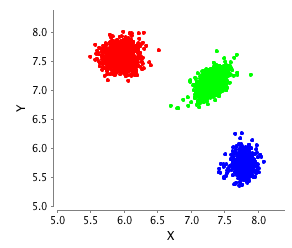
\epsfig{file=good4_cropped.png,width=0.5\linewidth,clip=} &
		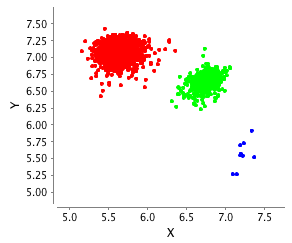
\epsfig{file=good5_cropped.png,width=0.5\linewidth,clip=} \\
	\end{tabular}
	\caption{An example of two good intensity cluster plots.}
	\label{good}
\end{figure}

\subsection{Easy to call SNPs which are called poorly}
In these examples, the clouds are clear, but the genotyping algorithm has made obvious mistakes in assigning genotypes (figure \ref{bad1}).
\begin{figure}[H]
	\centering
	\begin{tabular}{cc}
		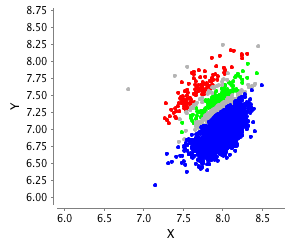
\epsfig{file=bad5_cropped.png,width=0.5\linewidth,clip=} &
		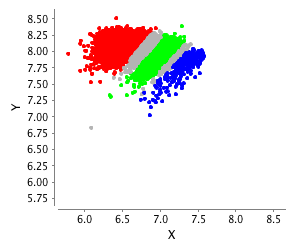
\epsfig{file=bad_cropped.png,width=0.5\linewidth,clip=} 
	\end{tabular}
	\caption{Two examples of intensity cluster plots showing good clusters that have been poorly called.}
	\label{bad1}
\end{figure}

\subsection{Hard to call SNPs}
Some SNPs simply don't have well defined clusters, or have $>$ 3 clusters, making them difficult to call even with a perfect genotyping algorithm. Examples of such SNPs are shown in figure \ref{bad2}, but it is important to remember that different platforms can produce a wide variety of bad clusters.
\begin{figure}[H]
	\centering
	\begin{tabular}{cc}
		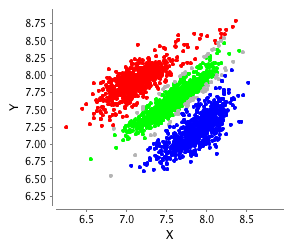
\epsfig{file=bad4_cropped.png,width=0.5\linewidth,clip=} &
		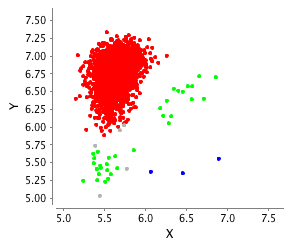
\epsfig{file=bad7_cropped.png,width=0.5\linewidth,clip=}
	\end{tabular}
	\caption{Two examples of intensity clusters plots with poorly defined clusters.}
	\label{bad2}
\end{figure}
 
\section{Additional Resources and tips}

\subsection{The binary intensity format}

The binary intensity format is very simple. First, a `magic number' of two bytes is written to the beginning of the file so that Evoker can recognise it. These bytes for Evoker are:
\begin{verbatim}
00011010 00110001
\end{verbatim}

\noindent After these, each point is stored as a pair of 4--byte floats (for the intensity of the two alleles). These are simply packed in the same order as the text intensity files described above (a pair for each individual for the first SNP, then the same for the second SNP and so on).

Evoker can also accept binary intensity data that uses two four byte integer values representing the number of rows of data (SNPs) and the number of columns (samples) as a header.

\subsection{Tips}

The perl scripts included are intended to work in most UNIX environments. They assume that the perl executable can be found in your path.  Also, make sure that the script is `world executable'. You can accomplish this with the following command: 

\begin{verbatim}
chmod +x evoker-helper.pl
\end{verbatim}

\noindent An easy way to get the correct string to enter in the data connection dialog for the remote directory is to login to that machine, change to that directory and run the \texttt{pwd} command, which will print the absolute path to that directory, which you can then cut and paste into the Evoker window.

\noindent While Evoker will handle Oxford format data which is compressed (files ending \texttt{.gz}), the program will be far more responsive if you unzip all compressed files.

\noindent In order to achieve consistent coloring of clusters across collections requires that for each SNP the alleles in each collection \texttt{.bim} file are in the same order.

\subsection{Resources}
Evoker.jar requires Java 5.0 or newer to run. You can download the latest version of Java at \texttt{www.java.com}
\\
\\
\texttt{PLINK} binary pedfile (\texttt{.bed}) format:  

\indent \texttt{http://pngu.mgh.harvard.edu/purcell/plink/data.shtml\#bed}
\end{document}